\documentclass[12pt, letterpaper]{article}
\usepackage[margin=1in]{geometry}
\usepackage{amsmath,amsthm,array, amssymb,amsfonts, cancel, enumitem, fancyhdr, color, comment, graphicx, environ}

\setlist[description]{leftmargin=\parindent,labelindent=\parindent}

\author{Val Anthony Balagon}
\date{February 2019}
\title{Chapter 5: Determinants}

%User commands
\newcommand{\R}[1]{$\mathbb{R}^{#1}$}
\newcommand{\Vector}[1]{$\textbf{#1}$}
\newcommand{\V}[1]{\textbf{\textit{#1}}}
\newcommand{\inverse}[1]{#1^{-1}}
\newcommand{\DefinitionSpace}{\vspace{15px}}


\newtheorem*{remark}{Remark}

\theoremstyle{definition}
\newtheorem{definition}{Definition}[section]

\newtheorem{example}{Example}
\newtheorem{theorem}{Theorem}

\newcommand*{\vertbar}{\rule[-1ex]{0.5pt}{2.5ex}}



\newenvironment{problem}[2][Problem]{\begin{trivlist}
		\item[\hskip \labelsep {\bfseries #1}\hskip \labelsep {\bfseries #2.}]}{\end{trivlist}}



\begin{document}
	\maketitle
	\begin{abstract}
		This chapter focuses on properties, and methods on computing determinants.
	\end{abstract}

\section{Properties of Determinants}
	Any square matrix, invertible or not, has a special number that contains a lot of information called the \textbf{determinant}. It tells immediately if a matrix is invertible or not since \textbf{a singular matrix has a determinant of zero}. When $A$ is invertible, the determinant of $A^{-1}$ is $\frac{1}{\det(A)}$. There are three common ways to compute for the determinant. These are the following:
	
		{\centering
			\begin{enumerate}
				\item Pivot formula
				\item ``Big" formula
				\item Cofactor formula
		\end{enumerate}}
	
	\noindent The determinant is written in 2 ways, $\det(A) \text{ and } |A|$. The determinant of \[A \begin{bmatrix} a & b \\ c & d \end{bmatrix} \text{\quad is\quad} \begin{vmatrix}a & b \\ c & d\end{vmatrix} = ad - bc.\]
	
\paragraph{Property 1}
Determinant of a square identity matrix is 1.
	\[\det{I} = 1 \text{\quad and\quad} \begin{vmatrix}
									1   &   & \\
									& \ddots& \\
									&       & 1 
								\end{vmatrix} = 1\]

\DefinitionSpace
\paragraph{Property 2}
The determinant changes sign when two rows are exchanged.
	\[\begin{vmatrix}
		c & d\\
		a & b
	 \end{vmatrix} = - \begin{vmatrix}
						 a & b \\
						 c & d
						 \end{vmatrix}\]
	\begin{example}
		\[
		\begin{vmatrix}
		1 & 0 \\
		0 & 1
		\end{vmatrix} = 1 \rightarrow \begin{vmatrix}
										0 & 1 \\
										1 & 0
										\end{vmatrix} = -1
										\]
	\end{example}
	In the earlier chapters, we know that row exchanges can be performed by multiplying matrix $A$ with a permutation matrix $P$. $\det(P) = +1$ for \textbf{even} number of row exchanges and $\det(P) = -1$ for \textbf{odd} row exchanges.
	
\DefinitionSpace
\paragraph{Property 3}
The determinant is a linear function or operator for each row. If the first row is multiplied by $t$, the determinant is multiplied by $t$.
	\begin{example}
		\begin{gather*}
			\begin{vmatrix}
				ta & tb \\
				c & d		
			\end{vmatrix} = tad - tbc = t(ad - bc) = t \begin{vmatrix}
														a & b \\
														c & d		
														\end{vmatrix}
		\end{gather*}
	\end{example}
	
	
	\begin{example}
		\begin{gather*}
			\begin{vmatrix}
				a+a' & b+b' \\
				c & d		
			\end{vmatrix} = (a+a')d - (b+b')c = (ad-bc) + (a'd - b'c) = \begin{vmatrix}
																			a & b \\
																			c & d		
																			\end{vmatrix} + \begin{vmatrix}
																								a' & 'b \\
																								c & d		
																								\end{vmatrix}
		\end{gather*}
	\end{example}

	\begin{example}
		\begin{align*}
			\begin{vmatrix}
				a+a' & b+b' \\
				tc & td		
			\end{vmatrix} &= (a + a')td - (b + b')tc \\
			              &= t\left[ ad + a'd - bc - b'c \right] \\
			              &=  t\left[ (ad- bc)  + (a'd - b'c )\right]
		\end{align*}
	\end{example}

	\begin{gather*}
		\det(A^2) = (\det(A))^2 \\
		\det(2A) = 2^n \det(A)
		\end{gather*}

\DefinitionSpace
\paragraph{Property 4}
If two rows are equal, the determinant is zero.
	\begin{example}
		\begin{gather*}
			\begin{vmatrix}
				a & b \\
				a & b 
			\end{vmatrix} = ab - ab = 0
		\end{gather*}
	\end{example}

	If we perform a row exchange we still get the same matrix but because of rule 2 the determinant must change signs. We get $-D = D$, and the only way that this is consistent is when $D = 0$. A matrix with two equal rows has no inverse (matrix is singular). 
	
	
\DefinitionSpace
\paragraph{Property 5}
Elimination from $A$ to $U$ does not change the value of the determinant. Hence $\det(A) = \det(U)$.

	\begin{example}
		\begin{align*}
			\begin{vmatrix}
				a & b\\
				c - la & d - lb
			\end{vmatrix} &= a(d - lb) - b(c - la) \\
						  &= ad - \cancel{alb} - bc + \cancel{alb} \\
						  &= ad - bc \\
						  &= \begin{vmatrix}
						  			a & b\\
						  			c & d
						     \end{vmatrix}
		\end{align*}
	\end{example}


\DefinitionSpace
\paragraph{Property 6}
A matrix with a row of zeros has a determinant of zeros.

\DefinitionSpace
\paragraph{Property 7}
The determinant of an upper triangular matrix is the product of the diagonal entries.
	\begin{align*}
		U &= \begin{bmatrix}
				a_{11} & \dagger & \ldots & \dagger \\
				0   & \ddots  & \vdots & \dagger \\
				\vdots  & \ddots  & \ddots & \vdots \\
				0 & \ldots & 0  & a_{nn}
			\end{bmatrix} \\
		\det{U} &= \prod_{i=1}^{n} a_{ii}
	\end{align*}
	
	
To verify property 1, we simply multiply the diagonals of an identity matrix and $\det(I) = 1$. If there is a zero in the diagonal, then the determinant is zero. 

\DefinitionSpace
\paragraph{Property 8}
If $A$ is a singular matrix, then $\det(A) = 0$. If $A$ is invertible then $\det(A) \ne 0$. This is evident in singular matrices when we do elimination from $A$ to $U$ and we get a row of zeros and via rule 6 the determinant is zero. If $A$ is invertible then $U$ has pivots along its diagonal. The product of nonzero pivots gives a nonzero determinant.
	\begin{gather*}
		\det(A) = \pm \det(U) = \pm (\text{\textbf{product of the pivots}}) 
	\end{gather*}

\noindent The pivots of a $2\times2$ matrix are $a$ and $d - (c/a)b$.
	\begin{gather*}
			\begin{vmatrix}
				a & b\\
				c & d
				\end{vmatrix} = \begin{vmatrix}
									a & b\\
									0 & d - (c/a)b
									\end{vmatrix} = ad - bc
	\end{gather*} The sign in $\pm \det(U)$ depends on whether the number of row exchanges is even or odd: +1 or -1 is the determinant of the permutation $P$ that exchanges rows. With no row exchanges, $P = I$ and $\det(A) = \det(U)$.
		\begin{gather*}
			PA = LU \\
			\det(P) \det(A) = \det(L) \det(U)
		\intertext{$\det(P) = \det(I) = 1$ and $L$'s diagonal only contains ones, hence $\det(L)=1$.}
			\det(A) = \det(U)
		\end{gather*}


\DefinitionSpace
\paragraph{Property 9} The determinant of $AB$ is: \[\det(AB) = \det(A) \det(B).\] From this property, we can calculate the inverse.
	\begin{gather*}
		A A^{-1} = I \\
		\det(A)\det(A^{-1}) = 1 \\
		\boxed{\det(A^{-1}) = \frac{1}{\det(A)}}
	\end{gather*}
	
	To prove this property, suppose we have two $2\times2$ matrices $A$ and $B$.
		\[A = \begin{vmatrix}
				a & b\\
				c & d
				\end{vmatrix} \text{ \qquad } B = \begin{vmatrix}
														p & q\\
														r & s
														\end{vmatrix}\]
		\begin{align*}
			|A||B| &= (ad -bc)(ps - qr) \\
				   &= (ap + br)(cq + ds) - (aq+bs)(cp+dr) = |AB|
		\end{align*}	

\DefinitionSpace
\paragraph{Property 10}
The determinant of the transpose is equal to the determinant of the original matrix.
	\begin{gather*}
		\det(A^T) = \det(A) \\
	\end{gather*}
	
	\begin{proof}
		Say $A$ is invertible and we do not have any row exchanges, then $P = I$.
		\begin{gather*}
			PA = LU \\
			A^T P^T = U^T L^T \\
			\det(A^T)\det(P^T) = \det(U^T)\det(L^T)
		\intertext{$L^T$ has ones in the diagonal then its determinant is 1. Same with the determinant of $P^T$.}
			\det(A^T) = \det(U^T)
		\end{gather*}
		$U$ and $U^T$ have the same diagonals, therefore $A$ and $A^T$ have the same determinants.
	\end{proof}

	\begin{example}
		\begin{align*}
			\begin{vmatrix}
			a & c \\
			b & d
			\end{vmatrix} &= \begin{vmatrix}
								a & b\\ 
								c & d
								\end{vmatrix} \\
			ad - bc &= ad - bc
		\end{align*}
	\end{example}





\section{Inverses, Cramer's Rule, and Volumes}
\subsection{Inverse}
For the $2 \times 2$ case, the formula for the inverse of $A$ is \[ A^{-1} = \frac{1}{\det(A)}\begin{bmatrix}
																						d & -b \\
																						-c & a
																						\end{bmatrix}. \]For the $n \times n$ case, we have \[ A^{-1} = \frac{1}{\det(A)} C^{T} \]
																						
\subsection{Cramer's Rule}
To solve $A\V{x = \V{b}}$, we use $\V{x} = \inverse{A} \V{b}$. According to the last section, this formula is equivalent to \[\V{x} = \frac{1}{\det(A)} C^{T} \V{b}. \] 
	\DefinitionSpace
	\begin{definition}
		If $\det(A) \ne 0$, $A\V{x} = \V{b}$ is solvable using determinants:
			\begin{equation}
				\V{x}_1 = \frac{\det(B_1)}{\det(A)} \quad \V{x}_2 = \frac{\det(B_2)}{\det(A)} \quad \ldots \V{x}_n = \frac{\det(B_n)}{\det(A)}
			\end{equation}Where $B_i$ is \begin{equation*} B_i = \text{$A$ with column $i$ replaced by $\V{b}$}\end{equation*}
	\end{definition}
	\DefinitionSpace
Cramer's rule is an explicit formula for the solution $\V{x}$ but it involves way too many operations.	

	\begin{example}
		Solve for $x_1, x_2$:
			\[\begin{bmatrix}
				3 & 4 \\
				5 & 6
			 \end{bmatrix} \begin{bmatrix} x_1 \\ x_2\end{bmatrix} = \begin{bmatrix} 2 \\ 4\end{bmatrix}\] 
		\begin{gather*}
			\intertext{The determinant of $A$ is:}
				\det(A) = \begin{vmatrix}
								3 & 4 \\
								5 & 6
								\end{vmatrix} = 3\cdot 6 - 4\cdot 5 = -2
			\intertext{Solving for $x_1$:}
				x_1 = \frac{\det(B_1)}{\det(A)} = \frac{\begin{vmatrix}
					2 & 4 \\
					4 & 6
					\end{vmatrix}}{\det(A)} = \frac{2 \cdot 6 - 4 \cdot 4}{-2} = \frac{-4}{-2} = 2
			\intertext{Solving for $x_2$:}
				x_2 = \frac{\det(B_2)}{\det(A)} = \frac{\begin{vmatrix}
															3 & 2\\
															5 & 4
													\end{vmatrix}}{\det(A)} = \frac{3 \cdot 4 - 2 \cdot 5}{-2} = \frac{2}{-2} = -1
			\intertext{Hence,}
				\V{x} =\begin{bmatrix}
							2 \\ -1
							\end{bmatrix}
		\end{gather*}
	\end{example}

\subsection{Cross Product}

	\begin{definition}
		The cross product of $\V{u} = (u_1, u_2, u_3)$ and $\V{v} = (v_1, v_2, v_3)$ is a vector \begin{equation}
																									\V{u} \times \V{v} = \begin{vmatrix}
																															\V{i} & \V{j} &\V{k} \\
																															u_1 & u_2 & u_3 \\
																															v_1 & v_2 & v_3
																															\end{vmatrix} = 
																															(u_2v_3 - u_3v_2)\V{i} + 
																															(u_3v_1 - u_1v_3)\V{j} + 
																															(u_1v_2-u_2v_1)\V{k}.
																								\end{equation}
		Using the Levi-Civita symbol: \begin{equation*}
													\V{u} \times \V{v} = \sum_{i}\sum_{j}\sum_{k} \epsilon_{ijk} u_j v_k
											\end{equation*} This vector $\V{u} \times \V{v}$ is perpendicular to $\V{u}$ and $\V{v}$. The cross product $\V{v} \times \V{u}$ is $-(\V{u} \times \V{v})$.
	\end{definition}
	\DefinitionSpace
	
		\begin{figure}[h!]
			\centering
			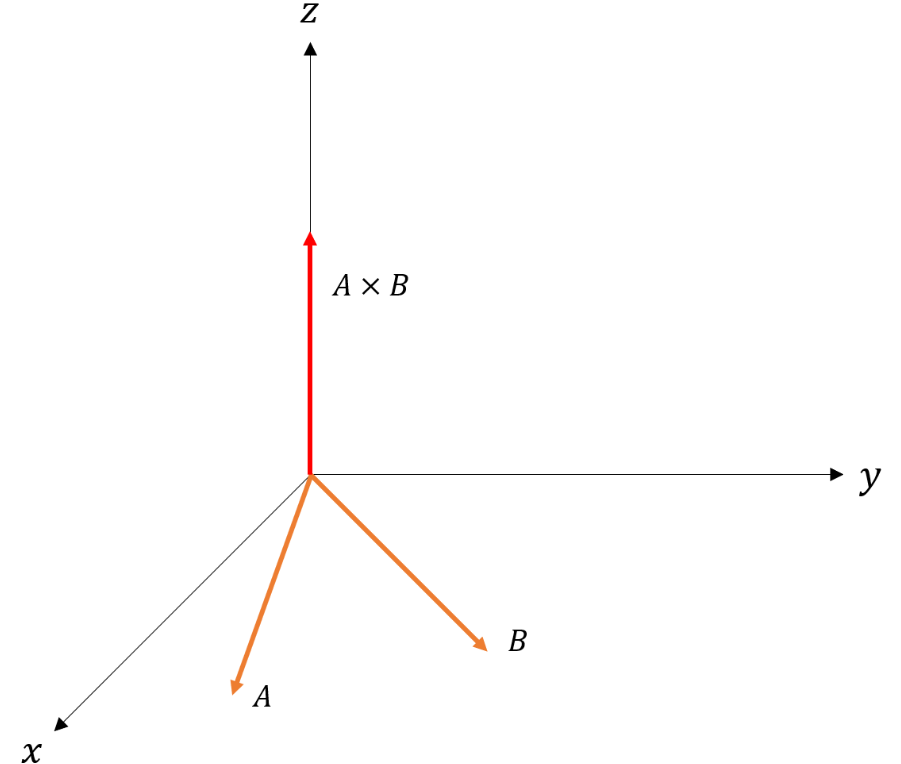
\includegraphics[scale=0.3]{crossproduct_geometry.png}
			\caption{Geometry of the cross product.}
			\label{cross_prod_geom}
		\end{figure}
		
	
\paragraph{Property 1} $\V{v} \times \V{u}$ reverses rows 2 and 3 in the determinant so it equals -($\V{u} \times \V{v}$).

\paragraph{Property 2} The cross product $\V{u} \times \V{v}$ is perpendicular to \V{v} and \V{u}.
	\begin{proof}
		\begin{equation*}
			\V{u} \cdot (\V{u} \times \V{v}) = u_1(u_2v_3 - u_3v_2) + u_2(u_3v_1 - u_1v_3) + u_3(u_1v_2 - u_2v_1) = 0
		\end{equation*}
	\end{proof}

\paragraph{Property 3} The cross product of any vector with itself is $\V{u} \times \V{u} = 0$. This is because the determinant has two equal rows. When $\V{u}$ and $\V{v}$ are parallel, their cross product is zero. When $\V{u}$ and $\V{v}$ are perpendicular, their dot product is zero.

	\begin{gather*}
		||\V{u} \times \V{v}|| =  ||\V{u}||||\V{v}|||\sin{\theta}|   \qquad ||\V{u} \cdot \V{v}|| = ||\V{u}||||\V{v}|||\cos{\theta}|
	\end{gather*}

\paragraph{Property 4} The length of $\V{u} \times \V{u}$ equals the area of the parallelogram with sides $\V{u}$ and $\V{v}$.

	\DefinitionSpace
	\begin{definition}
		The cross product is a vector with length $||\V{u}|| ||\V{v}|| |\sin{\theta}|$. Its direction is perpendicular to $\V{u}$ and $\V{v}$. It points up or down by the right hand rule.
	\end{definition}



\begin{example}
	Find $\V{u} \times \V{v}$ and $||\V{u} \times \V{v}||$ of $\V{u} = (1,1,1)$ and $\V{v} = (1,1,2)$.
		\begin{gather*}
		\V{u} \times \V{v} = \begin{vmatrix}
								\V{i} & \V{j} &\V{k} \\
								1 & 1 & 1 \\
								1 & 1 & 2
								\end{vmatrix} = \V{i}\begin{vmatrix}
													1 & 1 \\
													1 & 2
													\end{vmatrix} + \V{j}\begin{vmatrix}
																			1 & 1 \\
																			1 & 2
																			\end{vmatrix} + \V{k}\begin{vmatrix}
																									1 & 1 \\
																									1 & 1
																									\end{vmatrix} = \V{i} - \V{j} \\
		||\V{u} \times \V{v}|| = \sqrt{1^2 + (-1)^2 + 0^2} = \sqrt{2}
		\end{gather*}
\end{example}


\subsection{Scalar Triple Product}
	The triple product is \[ (\V{u} \times \V{v})\cdot\V{w}.\] It is a scalar because the answer is a number. The scalar triple product is a determinant - it gives the volume of a $\V{u}, \V{v}, \V{w}$ box. \[ (\V{u} \times \V{v})\cdot\V{w} = \begin{vmatrix}
																		 w_1 & w_2 & w_3 \\
																		 u_1 & u_2 & u_3 \\
																		 v_1 & v_2 & v_3
																		\end{vmatrix} = \begin{vmatrix}
																							u_1 & u_2 & u_3 \\
																							v_1 & v_2 & v_3 \\
																							w_1 & w_2 & w_3
																							\end{vmatrix}\]

When $\V{u}, \V{v}, \V{w}$ are on the same plane, \[ (\V{u} \times \V{v})\cdot\V{w} = 0.\]


\end{document}